\documentclass[11pt]{article}

\usepackage{graphicx}

\usepackage{array}

\usepackage{xcolor, colortbl}

\usepackage[a4paper,total={8in,10in}]{geometry}

\usepackage{mdframed}

\usepackage{mdwlist}

\usepackage{geometry}

\usepackage{marginnote}

\usepackage{multicol}

\usepackage{hyperref}


\begin{document}
\textit{Contact-9910988199}                                                 \hspace{2.5cm}\textit{E-mail: divyansh.sgs@gmail.com}\hspace{2.5cm}\textit{LinkedIn: http://bit.ly/2p2MgXg}                           
\begin{mdframed}[backgroundcolor=orange]
\begin{flushright}
\begin{Huge}
\color{white}{\fontfamily{pbk}\selectfont Divyansh}\color{gray}{\fontfamily{pbk}\selectfont\textbf{Malhotra}}
\end{Huge}
\end{flushright}
\end{mdframed}

\textit{Address: Flat -135, Sec-12, Pkt-2, Dwarka, New Delhi-110075}\hspace{2.5cm}\textit{Electronics and Communication Engineer}
\begin{figure}[ht]
\begin{minipage}[b]{0.45\linewidth}
\centering
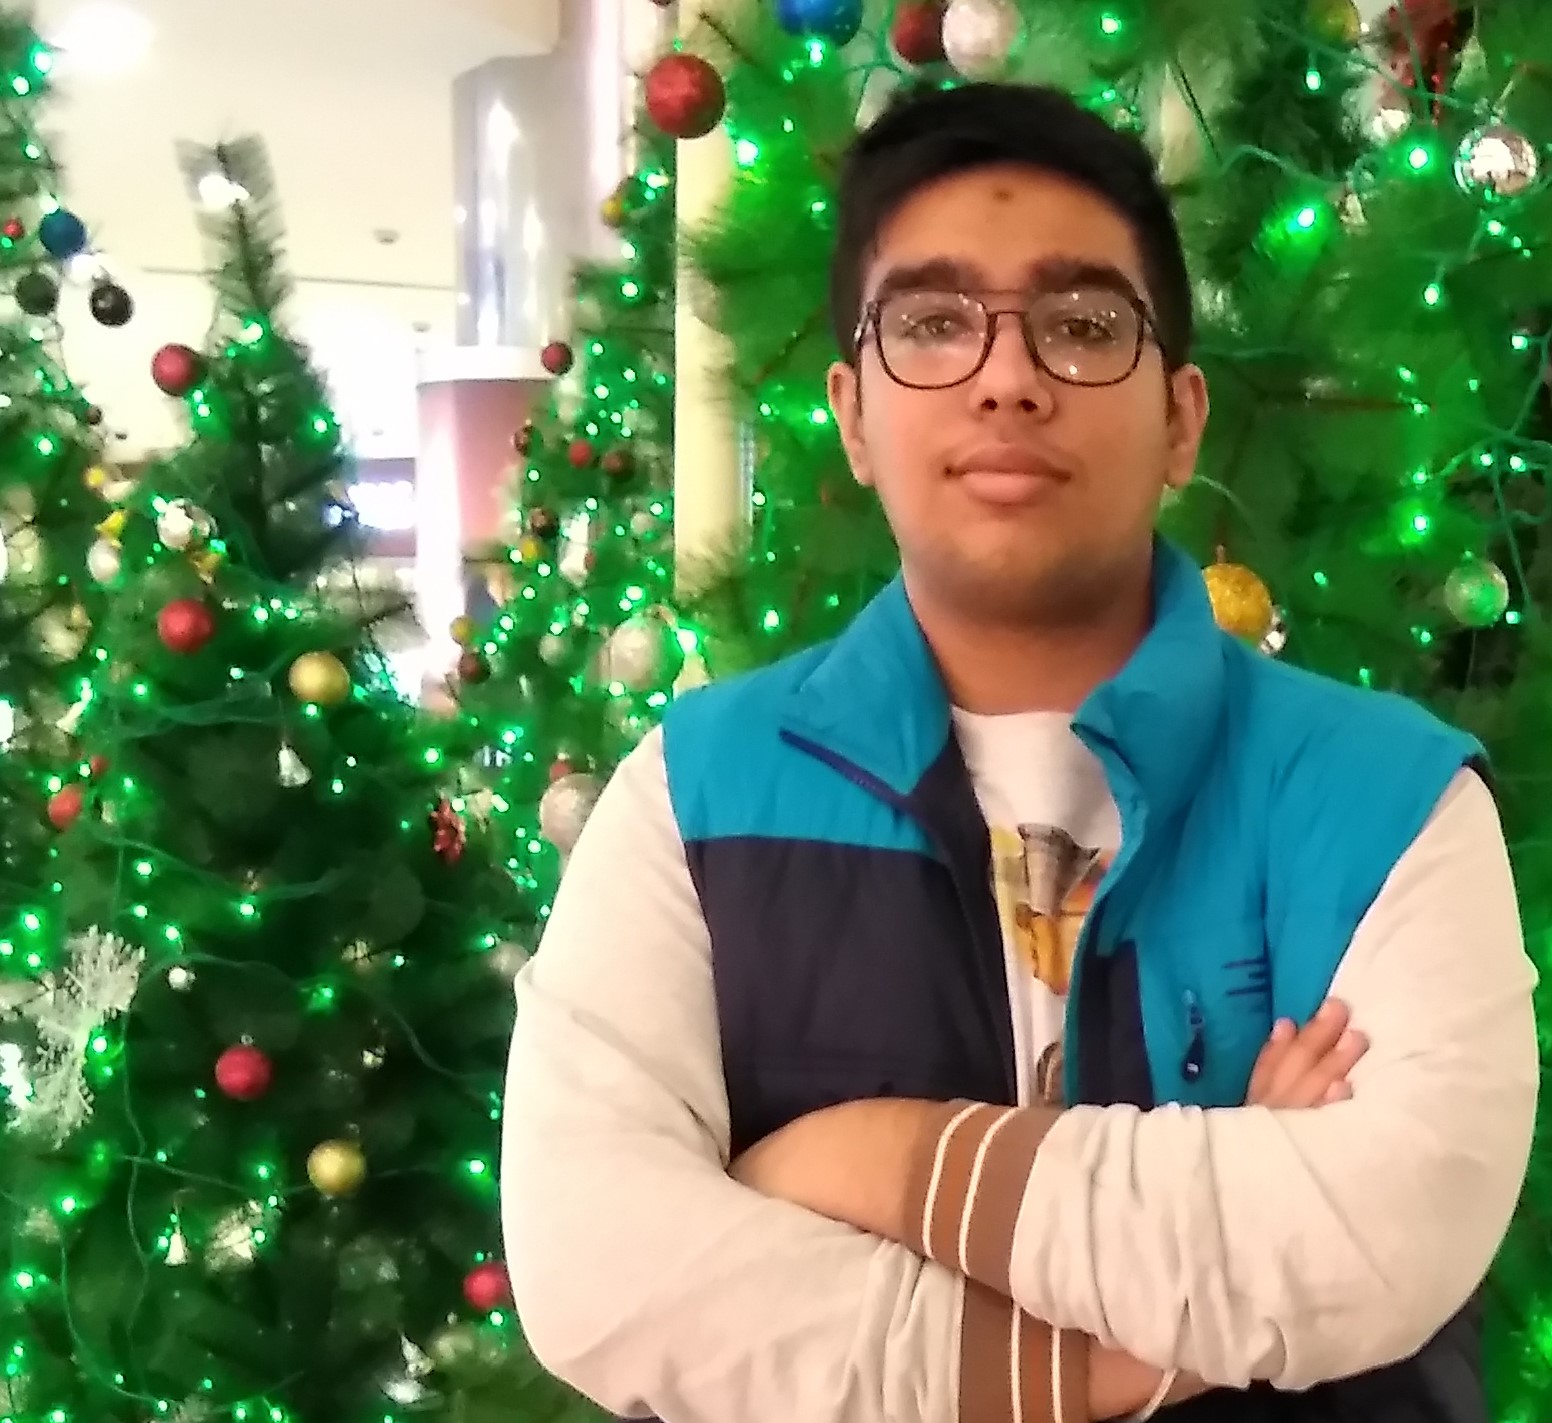
\includegraphics[scale=0.095]{photo2.jpg}
\end{minipage}
\hspace{0.5cm}
\begin{minipage}[b]{0.45\linewidth}
\flushleft
\begin{small}
I am an enthusiastic, imaginative and a full of energy student. I am a person who is open to all ideas, who hears all, analyses the data and then makes his own decisions. My nickname, as anointed by one of my professors, is the compiler because I tend to find the errors and work towards correcting them, not only in codes but also in life. I put my heart and soul into the work that I take up and am always eager to learn new skills everyday so that today, I can outshine my yesterday.\\
{\color{orange}{\textit{Career Objective:-} I am interested in coding and algorithm building. Thus, I intend to grow as a developer and see it as my future job.}}
\end{small}
\end{minipage}
\end{figure}\\
\begin{large}
\textsc{Education:-}
\end{large}
\definecolor{LightOrange}{rgb}{1,0.65,0}
\definecolor{WeakOrange}{rgb}{1,0.8,0.6}
\begin{center}
\begin{small}

\begin{tabular}{ |m{5.5cm} m{5.5cm} m{2cm} m{4.5cm}| }

\hline
\rowcolor{LightOrange}
\begin{center}

\textbf{{ Course/Examination }}

\end{center}&\begin{center}\textbf{ Institute/University }\end{center}&\begin{center}\textbf{ Year of passing }\end{center}&\begin{center}\textbf{ Performance }\end{center}\\

\hline

\begin{center}

B.Tech, Electronics and Communication Engineering

\end{center}& \begin{center}

Bharati Vidyapeeth's College Of Engineering

\end{center}&\begin{center}

2019

\end{center}& \begin{center}

76.57\%(Credited) (up to third semester)

\end{center}\\

\hline
\rowcolor{WeakOrange}
\begin{center}

AISSCE (SCIENCE-PCM with CS)\\

XIIth

\end{center}&

\begin{center}

(CBSE) Sachdeva Global School, New Delhi

\end{center}&

\begin{center}

2015

\end{center}&

\begin{center}

94.60 \%(agg)

\end{center}\\

\hline

\begin{center}

AISSE\\

Xth

\end{center}&

\begin{center}

(CBSE) Sachdeva Global School, New Delhi

\end{center}&

\begin{center}

2013

\end{center}&

\begin{center}

10 CGPA

\end{center}\\

\hline

\end{tabular}
\end{small}
\end{center}
\begin{figure}[ht]
\begin{minipage}[b]{0.45\linewidth}
\flushleft
\noindent\colorbox{WeakOrange}
{\parbox{\dimexpr\textwidth-2\fboxsep\relax}{\textsc{Projects:-}}}\\
%\textsc{Projects:-}\\
\begin{small}
\begin{enumerate}
\item  	Swarm Robotics
\item  Note identification using Python
\item  DTMF controlled home automation
\item  Developing a vehicle safety and caution system for highways under Celistini (Digital Image Processing) by Princeton University (February 2017- present)
\item 	Visible Light Communication(October 2016-Present)
\item 	Line Follower, Differential Drive Robot (Bluetooth Controlled) and other projects using AtMega16 and Arduino
\item  Android development – Calculator App that implements DMAS and an Anagrams game
\item  A model of a self-sustaining house
\end{enumerate}
\end{small}
\end{minipage}
\hspace{0.5cm}
\begin{minipage}[b]{0.45\linewidth}
\noindent\colorbox{WeakOrange}
{\parbox{\dimexpr\textwidth-2\fboxsep\relax}{\textsc{Training and Internship-}}}
%\textsc{Training and Internship:-}
\begin{small}
\begin{itemize}
\item  	Applied CS with android by GDG-BVP and Google
\item 	1- day Competitive Coding workshop by Hackaveda
\item 	1- day Git workshop by GDG- BVP
\item 	Series of Workshops on Arduino by IEEE RAS
\item	Series of Workshops on Competitive Coding by GDG-BVP
\item 	Android development for Beginners by Udacity(GDG)
\item 	 Ultimate Java Development Guide by Eduonix Learning Solutions
\item 	Workshop  on Embedded Systems by CETPA
\item 	Embedded Systems Summer Training by Cyborg Labs
\item Undertook an initiative to teach Java in the college
\end{itemize}
\end{small}
\flushleft


\end{minipage}
\end{figure}

\begin{figure}[ht]
\begin{minipage}[b]{0.45\linewidth}
\flushleft
\noindent\colorbox{WeakOrange}
{\parbox{\dimexpr\textwidth-2\fboxsep\relax}{\textsc{Research Publications:-}}}\\
\begin{small}
None. yet, but am currently working on Visible Light Communication and a Caution system for vehicles at highways.
\end{small}
\noindent\colorbox{WeakOrange}
{\parbox{\dimexpr\textwidth-2\fboxsep\relax}{\textsc{Technical Skills:-}}}\\
\begin{small}
\begin{enumerate}
\item  	Languages:
\begin{itemize}
\item C++
\item C
\item SQL
\item Java
\item XML
\item Python
\item Embedded C
\item 8085 instruction code
\item LaTex
\end{itemize}
\item  Operating Systems:
\begin{itemize}
\item Windows XP/7/8/10
\item Android
\end{itemize}
\item  Software and Platforms worked on:

\begin{itemize}
\item Microsoft Office
\item Photoshop CS6 and CS5
\item Arduino IDE
\item Audacity
\item AndroidStudio
\item Eclipse
\item Sony VegasPro
\item AfterEffects CS6
\item  Microsoft FrontPage
\item OpenOffice

\item  Turbo C++
\item CodeBlocks
\item  Orcad PSpice
\item AVR Studio 4
\item PROTEUS(ISIS and ARES)
\item XCTU
\item Python 2.x, Python 3.x
\item Autodesk Sketchbook
\item GNU Sim 8085
\item MATLAB
\item  ideone
\item  DevC++
\end{itemize}


\end{enumerate}
\end{small}
\end{minipage}
\hspace{0.5cm}
\begin{minipage}[b]{0.45\linewidth}
\noindent\colorbox{WeakOrange}
{\parbox{\dimexpr\textwidth-2\fboxsep\relax}{\textsc{Soft Skills-}}}

\begin{small}
\begin{itemize}
\item:Good Speaking Skills
\end{itemize}
\end{small}
\flushleft


\end{minipage}
\end{figure}
\end{document}